%% 
%% Copyright 2007-2019 Elsevier Ltd
%% 
%% This file is part of the 'Elsarticle Bundle'.
%% ---------------------------------------------
%% 
%% It may be distributed under the conditions of the LaTeX Project Public
%% License, either version 1.2 of this license or (at your option) any
%% later version.  The latest version of this license is in
%%    http://www.latex-project.org/lppl.txt
%% and version 1.2 or later is part of all distributions of LaTeX
%% version 1999/12/01 or later.
%% 
%% The list of all files belonging to the 'Elsarticle Bundle' is
%% given in the file `manifest.txt'.
%% 
%% Template article for Elsevier's document class `elsarticle'
%% with harvard style bibliographic references

%%\documentclass[preprint,12pt,authoryear]{elsarticle}

%% Use the option review to obtain double line spacing
%% \documentclass[authoryear,preprint,review,12pt]{elsarticle}

%% Use the options 1p,twocolumn; 3p; 3p,twocolumn; 5p; or 5p,twocolumn
%% for a journal layout:
%% \documentclass[final,1p,times,authoryear]{elsarticle}
%% \documentclass[final,1p,times,twocolumn,authoryear]{elsarticle}
%% \documentclass[final,3p,times,authoryear]{elsarticle}
%% \documentclass[final,3p,times,twocolumn,authoryear]{elsarticle}
%% \documentclass[final,5p,times,authoryear]{elsarticle}
\documentclass[final,5p,times,twocolumn,authoryear]{elsarticle}

%% For including figures, graphicx.sty has been loaded in
%% elsarticle.cls. If you prefer to use the old commands
%% please give \usepackage{epsfig}

%% The amssymb package provides various useful mathematical symbols
\usepackage{amssymb}
\usepackage{amsmath}
%% The amsthm package provides extended theorem environments
%% \usepackage{amsthm}
\usepackage{aas_macros}
%% The lineno packages adds line numbers. Start line numbering with
%% \begin{linenumbers}, end it with \end{linenumbers}. Or switch it on
%% for the whole article with \linenumbers.
%% \usepackage{lineno}

\journal{Astronomy and Computing}

\begin{document}

\begin{frontmatter}

%% Title, authors and addresses

%% use the tnoteref command within \title for footnotes;
%% use the tnotetext command for theassociated footnote;
%% use the fnref command within \author or \address for footnotes;
%% use the fntext command for theassociated footnote;
%% use the corref command within \author for corresponding author footnotes;
%% use the cortext command for theassociated footnote;
%% use the ead command for the email address,
%% and the form \ead[url] for the home page:
%% \title{Title\tnoteref{label1}}
%% \tnotetext[label1]{}
%% \author{Name\corref{cor1}\fnref{label2}}
%% \ead{email address}
%% \ead[url]{home page}
%% \fntext[label2]{}
%% \cortext[cor1]{}
%% \address{Address\fnref{label3}}
%% \fntext[label3]{}

\title{jax-cosmo: End-to-End Differentiable and GPU Accelerated Cosmology Library}

%% use optional labels to link authors explicitly to addresses:
%% \author[label1,label2]{}
%% \address[label1]{}
%% \address[label2]{}

\author{jax-cosmo contributors}

\address{}

\begin{abstract}
With jax-cosmo, Fisher forecasts are accurate and instantaneous, inference is lightning-fast, survey optimization is trivial.
\end{abstract}

%%Graphical abstract
%\begin{graphicalabstract}
%\includegraphics{grabs}
%\end{graphicalabstract}

%%Research highlights
%\begin{highlights}
%\item Research highlight 1
%\item Research highlight 2
%\end{highlights}

\begin{keyword}
%% keywords here, in the form: keyword \sep keyword

%% PACS codes here, in the form: \PACS code \sep code

%% MSC codes here, in the form: \MSC code \sep code
%% or \MSC[2008] code \sep code (2000 is the default)

\end{keyword}

\end{frontmatter}

%% \linenumbers

%% main text

\section{Introduction}



\section{JAX: Autograd meets XLA}


\section{Architecture}


\section{Validation against the Core Cosmology Library (CCL)} 

\section{Example of applications}

\subsection{Instantaneous Fisher Forecasts}


\subsection{Survey Optimization by FoM Maximization}


\subsection{Massive Optimal Compression in 3 Lines}

\subsection{Efficient sampling in high dimensions with Hamiltonian Monte Carlo}

Hamiltonian Monte Carlo (HMC) is an MCMC-type method particularly suited to drawing
samples from high dimensional parameter spaces.  It was introduced in \citet{duane}
and developed extensively since.  See \citet{betancourt} for a full review; we describe
very basic features here.

HMC samples spaces by generating particle tracjectories through the space, using the log-posterior
as the negative potential energy of a particle at each point $q$ in the space.  At each sample a trajectory are initialized
with a random momentum $p$, and then integrated using Hamilton's equations with a numerical integration:
\begin{align}
\frac{\mathrm{d}p}{\mathrm{d}t} &= - \frac{\partial V}{\mathrm{d} q} = \frac{\partial \log{\cal P}}{\mathrm{d} q}\\
\frac{\mathrm{d}q}{\mathrm{d}t} &= + \frac{\partial U}{\mathrm{d} p} = M^{-1} p
\end{align}
where $M$ is a mass matrix which should be set to approximate the covariance of the posterior. This is also
used to set the scale of the random initial velocities.

Formally, the set of $n_\mathrm{dim}$ moment are treated as new parameters, and after 
some number of integration steps a final point in the trajectory is compared to the initial one,
and a Metropolis-Hastings acceptance criterion on the total energy $H = p^T M^{-1} p + \log{\cal P}(q)$ is applied.
If the trajectory is perfectly simulation then this acceptance is unity, since energy is conserved; applying it allows
a relaxation to the integration accuracy.

That gradients $\partial \log{\cal P} / \mathrm{d} q$ can be estimated using finite differencing,
but this typically requires at least $4 n_{\mathrm{dim}} + 1$ posterior evaluations per point, greatly slowing it
in high dimension, and as with the Fisher forecasting is highly prone to numerical error. Automatically
calculating a Hessian, as in JAX-Cosmo, makes it feasible and efficient.

Below we show an example set of HMC constraints using JAX-Cosmo to constrain a simulated
Dark Energy Survey Year One (DES-Y1) lensing and clustering-like (3x2pt) likelihood, using 21 parameters\footnote{We omit the 
five clustering sample photometric redshift parameters}.  We re-parametrize the space to unit mass using the Cholesky 
decomposition
of the covariance as estimated with an initial Fisher matrix; this lets us reflect the trajectories when they reach the
edge of the parameter space, as recommended in \citet{afshar}.  We use a fixed number (25) of integration steps and 
a fixed integration period (0.02), this was chosen heuristically to give a reasonable acceptance rate, but is likely to be
far from optimal.  We compare to the highly-optimized {\sc Cobaya} 
Metropolis-Hastings implementation \citep{cobaya2,cobaya1}, initializing it with the Fisher matrix as a proposal and
tuning thereafter.  We ran two processes for each sampler, with four CPU threads per process.

The Hamiltonian sampler required around half the number of samples as the Metropolis (70,000 vs 140,000) to reach approximately the same
convergence, as tested by the Gelman-Rubin test \citep{gelman}, though each sample was itself a few times slower
on a CPU.  This proof-of-principle example can certainly be hugely improved using various extensions to HMC such as No U-Turn Sampling \citep{nuts} or sampling from the entire trajectories \cite{betancourt}.  On next generation GPU high-performance systems, the advantage will be large.

\begin{figure}
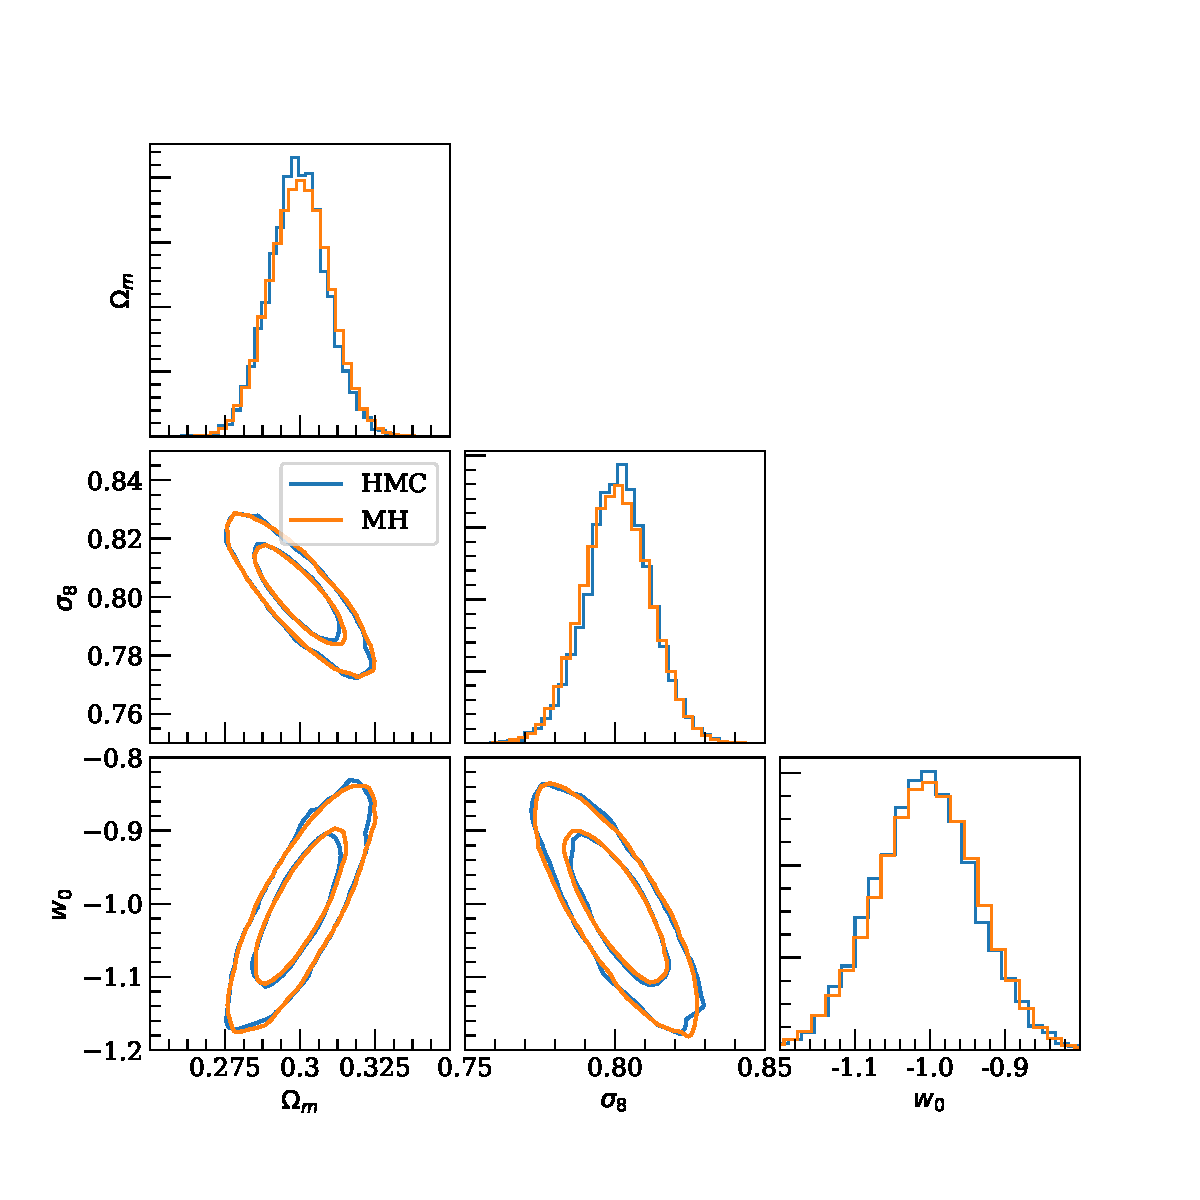
\includegraphics[width=0.95\columnwidth]{figures/hmc.pdf}
\caption{Constraints on three of the 21 parameters of a simulated DES-Y1 3x2pt likelihood, using a simple Hamiltonian
Monte Carlo sampler with JAX-Cosmo (blue), compared to the Cobaya Metropolis-Hastings sampler (orange).}
\end{figure}


We note that a full Boltzmann code accurate enough to calculate the CMB spectra to Planck \citep{planck18}
or future \citep{s4,simons} accuracy is currently beyond the scope of this project.  
If this is needed then HMC could use a fast approximation to a CMB theory spectrum, and importance sampling applied to the complete chain.


\subsection{Lightning fast inference with BayesFast}


%% The Appendices part is started with the command \appendix;
%% appendix sections are then done as normal sections
%% \appendix

%% \section{}
%% \label{}

%% If you have bibdatabase file and want bibtex to generate the
%% bibitems, please use
%%
\section*{Bibliography}
\bibliographystyle{elsarticle-harv} 
\bibliography{refs}

%% else use the following coding to input the bibitems directly in the
%% TeX file.

\end{document}

\endinput
%%
%% End of file `elsarticle-template-harv.tex'.